\lhead{\begin{tikzpicture}[remember picture, overlay]
    \node [anchor=100,inner sep=0] (imagenIZQUIERDA) at (current page header area.north){
\includegraphics[width=18cm]{img/Encabezado.PNG}};
    \end{tikzpicture}}
    \rhead{Ángeles-Hurtado}
    \rfoot{\begin{tikzpicture}[remember picture, overlay]
    \node [anchor=140,inner sep=0] (imagenDERECHA) at (current page footer area.south){
\includegraphics[width=18cm]{img/Foot.PNG}};
    \end{tikzpicture}}
    %----------------------------------------------------------------------------------------
    \lfoot{ \thepage}
    % \renewcommand{\labelenumi}{\alph{enumi}.)} 
    %----------------------------------------------------------------------------------------
    %----------------------------------------------------------------------------------------
    %	TITLE SECTION
    %----------------------------------------------------------------------------------------
    
    \setlength{\droptitle}{-5\baselineskip} % Move the title up
    \title{\textbf{Estudio de tiempos y movimientos en el ensamble de un circuito electrónico utilizando diferentes métodos para su optimización }} % Article title
    
     \author{ 
     \textsc{Piedra Moreno, Luis Angel}\\ 
    %  Afiliación:
     \texttt{ Instituto Tecnológico de Querétaro } \\ 
     \texttt{ Tecnológico Nacional de México } \\ 
     \texttt{Querétaro, México}\\ 
     \texttt{lc18141014@queretaro.tecnm.mx} 
     \and 
     \textsc{Ángeles-Hurtado, Luis Alberto}\\ 
    %  Afiliación:
     \texttt{ Instituto Tecnológico de Querétaro } \\ 
     \texttt{ Tecnológico Nacional de México } \\ 
     \texttt{Querétaro, México}\\ 
     \texttt{alb3rt0.ah@gmail.com} 
    }
    
    
    %----------------------------------------------------------------------------------------
    
    % \begin{document}
    
    % Print the title
    \maketitle
    \thispagestyle{fancy}
    
    %----------------------------------------------------------------------------------------
    %	ARTICLE CONTENTS
    %----------------------------------------------------------------------------------------
    
    % \section*{Resumen}
    % \textit{Palabras clave:}
    % El resumen (ancho de página) deberá contener entre 100 y 200 palabras tipo Adobe Devangari 11 puntos.
    
    \begin{abstract}
    \noindent 
    El resumen (ancho de página) deberá contener entre 100 y 200 palabras tipo Adobe Devangari 11 puntos.
    
    \end{abstract}
    % 
    % 
    \textbf{\textit{Palabras clave}}: {First keyword should be the corresponding to the research area according with the authors guide. Maximum of 6 keywords.}
    % \keywords{First keyword should be the corresponding to the research area according with the authors guide. Maximum of 6 keywords.}
    
    \section{Introducción}
    
    % Define estudio de tiempos y movimientos
    % define que es ensamble
    % define que es circuito electronico
    % define el metodo de tiempos predeterminados
    % define optimización
    \begin{itemize}
    
     \item El estudio de tiempos y movimientos es una herramienta fundamental para analizar y optimizar procesos de trabajo, especialmente en entornos de producción y ensamblaje. En este documento, se lleva a cabo un análisis de los tiempos y movimientos involucrados en el ensamblaje de un circuito electrónico compuesto por una pantalla LCD, un potenciómetro y una ESP32.
    
     \item El objetivo principal de este estudio es identificar oportunidades para mejorar la eficiencia del proceso de ensamblaje, reducir tiempos de operación y maximizar la productividad. Para lograrlo, se utilizarán diversas metodologías como el estudio de tiempos, análisis de movimientos y estudio de métodos.
    
     \item Además, se explorarán los avances recientes en la tecnología de circuitos electrónicos y en las técnicas de optimización del trabajo, con el fin de proponer mejoras innovadoras que contribuyan a la optimización del proceso de ensamblaje.
    
     \item Este documento tiene como meta ofrecer un análisis detallado y práctico que sirva de base para la toma de decisiones informadas sobre cómo mejorar la eficiencia y eficacia en el ensamblaje de circuitos electrónicos.
    
    
    \end{itemize}
    % 
    % 
    \section{Justificación}
    
    El estudio de tiempos y movimientos en el ensamblaje de circuitos electrónicos es un campo en constante evolución que responde a las demandas de eficiencia y productividad en la industria. En un contexto global, las empresas buscan optimizar sus procesos de ensamblaje para mantenerse competitivas en el mercado poniendo de ejemplo el ensamblaje de circuitos electrónicos es una parte crucial de numerosas industrias, desde la electrónica de consumo hasta la automotriz y la aeroespacial. En la actualidad, la demanda se centra en la eficiencia, la precisión y la flexibilidad en el proceso de ensamblaje.
    \begin{itemize}
    
    \item Reducción de costos:
        Las empresas buscan minimizar los costos de producción a través de la optimización de procesos.Esto incluye la reducción de tiempos de ciclo y la minimización de desperdicios.
    
    \item Capacitación y desarrollo de la fuerza laboral:
        Los trabajadores deben ser capacitados en técnicas de estudio de tiempos y movimientos para maximizar su productividad ya que igualmente la inversión en formación y desarrollo es esencial para mantener a los empleados actualizados con las últimas tecnologías y prácticas.
    
        \item https://ciateq.repositorioinstitucional.mx/jspui/handle/1020/729
        
    \end{itemize}
    % 
    % 
    \section{Descripción del problema}
    
    El proceso de ensamblaje de circuitos electrónicos en la actualidad enfrenta desafíos significativos en términos de eficiencia y productividad. Los operadores a menudo deben seguir instrucciones complejas y poco claras, lo que conduce a inconsistencias en la calidad del ensamblaje y tiempos de ciclo más largos de lo necesario. 
    
    \begin{itemize}
        \item Incógnita científica:
    Una de las incógnitas científicas clave es cómo optimizar el proceso de ensamblaje proporcionando instrucciones claras y sencillas a los operadores, lo que podría mejorar la eficiencia y calidad del ensamblaje de circuitos electrónicos. Además, se investiga cómo el análisis de tiempos y movimientos puede contribuir a identificar y eliminar ineficiencias en el proceso.
    
       
    \end{itemize}
    
    \textbf{*La incógnita científica es el elemento cuya solución incrementa el conocimiento científico.}
    % 
    % 
    \section{Fundamentación teórica}
    
    El estudio de tiempos y movimientos es una metodología bien establecida en el ámbito de la ingeniería industrial y de procesos, con el objetivo de optimizar la eficiencia y la productividad en diversas actividades, incluido el ensamblaje de circuitos electrónicos. A continuación, se presentan los conceptos clave, la hipótesis de tu proyecto, y las metodologías utilizadas.
    \begin{itemize}
        \item Estudio de tiempos y movimientos:
    
    El presente proyecto tiene como objetivo optimizar el proceso de ensamblaje de circuitos electrónicos mediante la aplicación de técnicas de estudio de tiempos y movimientos, la simplificación de instructivos y la optimización de métodos de trabajo. Para sustentar este proyecto, se presenta a continuación la condimentación teórica que enmarca los conceptos clave, la hipótesis de investigación y las metodologías a emplear.
        \item Estudio de Tiempos y Movimientos: Fundamentos y Objetivos
    
    El estudio de tiempos y movimientos (ETM) es una metodología ampliamente utilizada en el ámbito de la ingeniería industrial y de procesos, con el propósito de analizar y optimizar la eficiencia y productividad en diversas actividades, incluyendo el ensamblaje de componentes electrónicos. Esta técnica se basa en la medición y análisis rigurosos de los tiempos de ciclo de cada paso del proceso de producción, así como en la observación minuciosa de los movimientos que realizan los trabajadores durante el desempeño de sus tareas.
        \item Las estrategias clave para la optimización de procesos de ensamblaje incluyen:
    
    Estandarización de métodos: Establecer un método único y óptimo para realizar cada tarea de ensamblaje, garantizando la consistencia y la calidad en el proceso.
    Ergonomía y diseño del puesto de trabajo: Adaptar el entorno de trabajo a las necesidades físicas y cognitivas de los operadores, reduciendo la fatiga y mejorando el confort, lo que se traduce en un mejor desempeño.
    Capacitación y entrenamiento: Brindar a los operadores la formación adecuada en cuanto a las técnicas de ensamblaje correctas, el uso de herramientas y equipos, y la interpretación de instructivos claros.
        \item Metodologías de Investigación:
    
    Para llevar a cabo este estudio, se emplearán las siguientes metodologías de investigación:
    
    Estudio de tiempos: Se utilizarán técnicas de cronometraje y muestreo para medir y analizar los tiempos de ciclo de cada paso del proceso de ensamblaje.
    Análisis de movimientos: Se observarán y evaluarán los movimientos que realizan los operadores durante el ensamblaje, identificando movimientos ineficientes, cuellos de botella y oportunidades de mejora.
    Estudio de métodos: Se compararán diferentes enfoques de ensamblaje para determinar el método más eficiente, considerando factores como la ergonomía, la facilidad de comprensión de los instructivos y la calidad del producto final.
    \end{itemize}
    % 
    % 
    \section{Hipótesis}
    
    Es la suposición con fundamento científico relativa a la solución del problema, necesidad o de cómo se aprovecha la oportunidad con la incógnita científica y se fundamenta con: 1. Una suposición (en afirmativo o negativo) y ésta deberá vincularse con:
    2. La fundamentación científica que deberá ser precisa 3. Una entidad de comparación para probar la suposición y
    4. La variable con que se califica o cuantifica la comparación o se prueba la hipótesis.
    
    \begin{itemize}
        \item Se debe de identificar claramente la suposición científica
        \item Se debe de identificar claramente el fundamento científico
        \item Se debe identificar claramente la variable de respuesta
        \item Se debe identifican claramente las realidades o modelos contrastantes
        \item Se debe de establecer las variables asociadas, explicativas o que tienen relación funcional con la variable de respuesta
    \end{itemize}
    % 
    % 
    \section{Objetivo}
    
    Precisar la acción necesaria para probar la hipótesis. Dicha acción se establece mediante el uso de verbos activos y en infinitivo.
    \begin{itemize}
        \item Se debe establecer que se pretende probar la hipótesis
    \end{itemize}
    
    \subsection{Objetivos específicos }
    
    \begin{itemize}
        \item Se debe establecer como un conjunto de acciones comunes para lograr el objetivo general
        \item Se debe establecer como etapas para lograr el objetivo general
    \end{itemize}
    
    Son actividades orientadas al cumplimiento del objetivo general. Se establecen con verbos activos en infinitivo. Son parte de la acción encaminada a probar la hipótesis. Éstos deben ser precisos, y en lo posible evitar aspectos metodológicos.
    % 
    % 
    \section{Cuerpo (Metodología, modelo matemático, etc.)}
    
    Ensamblar un dispositivo electrónico compuesto por un tomacorriente, una tarjeta ESP32, una protoboard, un potenciómetro, una pantalla LCD y diversos cables. El dispositivo mostrará el mensaje "Hola mundo" en la pantalla LCD.
    
    \begin{itemize}
        \subsection{Herramientas y materiales}
        
        \item Multicontactos con 8 conectores de corriente, 3 conectores USB y 1 conector USB tipo C
        \item Tarjeta ESP32
        \item Protoboard
        \item Cables (macho-macho y macho-hembra)
        \item Potenciómetro
        \item Pantalla LCD  
    
        \subsection{1.- Preparación }
        \item Reúne todos los materiales y herramientas necesarias.
        \item Asegúrate de tener una superficie plana y bien iluminada para trabajar
    
        \subsection{2 Conexión a toma-corriente }
        \item Ubica los conectores del multi-contacto, encontrando la entrada del usb tipo c, el cual es el mas pequeño de todos.
        \item No es necesario conectar a la corriente electrica en este momento.
        \item Conecta el cable USB tipo C del multi-contacto al conector USB tipo C de la tarjeta ESP32.
    
        \subsection{3 Conexión de la protoboard }
        \item Ubica los pines de la protoboard.
        \item Coloca la tarjeta ESP32 sobre la protoboard, como se muestra en la imagen adjunta.
        \item Asegúrate de que las conexiones de los pines coincidan con la configuración de la protoboard.
         \item Presiona los pines de la tarjeta ESP32 sobre los pines de la protoboard para asegurar una conexión firme.
    
         \subsection{4 Conexión del potenciómetro }
        \item Ubica los pines del potenciómetro: 3 pines (generalmente marcados como VCC, GND y Signal).
        \item Conecta un cable jumper macho-macho al pin VCC del potenciómetro.
        \item Conecta otro cable jumper macho-macho al pin GND del potenciómetro.
        \item Conecta el cable jumper del pin VCC del potenciómetro al pin VCC en la protoboard (fila roja superior).
        \item Conecta el cable jumper del pin GND del potenciómetro al pin GND en la protoboard (fila azul superior).
         \item Conecta el cable jumper del pin Signal del potenciómetro al pin A0 en la protoboard (columna analógica izquierda).
    
          \subsection{5 Conexión del potenciómetro }
        \item Ubica los pines del potenciómetro: 3 pines (generalmente marcados como VCC, GND y Signal).
        \item Conecta un cable jumper macho-macho al pin VCC del potenciómetro.
        \item Conecta otro cable jumper macho-macho al pin GND del potenciómetro.
        \item Conecta el cable jumper del pin VCC del potenciómetro al pin VCC en la protoboard (fila roja superior).
        \item Conecta el cable jumper del pin GND del potenciómetro al pin GND en la protoboard (fila azul superior).
         \item Conecta el cable jumper del pin Signal del potenciómetro al pin A0 en la protoboard (columna analógica izquierda).
    
         \subsection{6 Conexión de la pantalla LCD}
        \item Ubica los pines de la pantalla LCD. La cantidad de pines puede variar, pero generalmente son 16 o más.
        \item Consulta la hoja de datos o documentación de la pantalla LCD para identificar los pines específicos.
        \item En la imagen adjunta, se muestra la conexión de una pantalla LCD común de 16 pines.
        \item Conecta los cables jumper a los pines correspondientes de la pantalla LCD, siguiendo el diagrama de pines proporcionado por el fabricante.
        \item Conecta el cable de alimentación VCC (generalmente marcado como VCC o +5V) de la pantalla LCD al pin VCC en la protoboard (fila roja superior).
         \item Conecta el cable de alimentación GND (generalmente marcado como GND) de la pantalla LCD al pin GND en la protoboard (fila azul superior).
          \item Conecta los cables de datos D0-D7 de la pantalla LCD a los pines digitales D2-D9 en la protoboard (fila azul central).
         \item Conecta el cable de control RS/EN (generalmente marcado como RS, EN o RW) de la pantalla LCD al pin D10 en la protoboard (fila azul central).
    
         \subsection{7 Prueba final }
        \item Enchufa el toma-corriente a una toma de corriente.
        \item Observa si la pantalla LCD muestra el mensaje "Hola mundo".
        \item Por ultimo mueve el potenciómetro verificando que todo esta en orden y esta completo el ensamble.
    
        \subsection{Errores}
        \item En caso que la pantalla LCD no arroje el mensaje "Hola mundo" hay que verificar que las conexiones están fijas.
        \item Revisar que los cables estén en su conexión correspondiente.
         \item Después de realizar las indicaciones anteriores ubicamos dos botones color negro en la ESP32 la cual presionamos el botón izquierdo el ya que es el botón de reste, posteriormente debería de funcionar correctamente.
    
        
        \item Se deben tener referencias Figura \ref{fig:lcd-16x2}.
    \end{itemize}
    % 
    % 
    \begin{figure}[H]
        \centering
        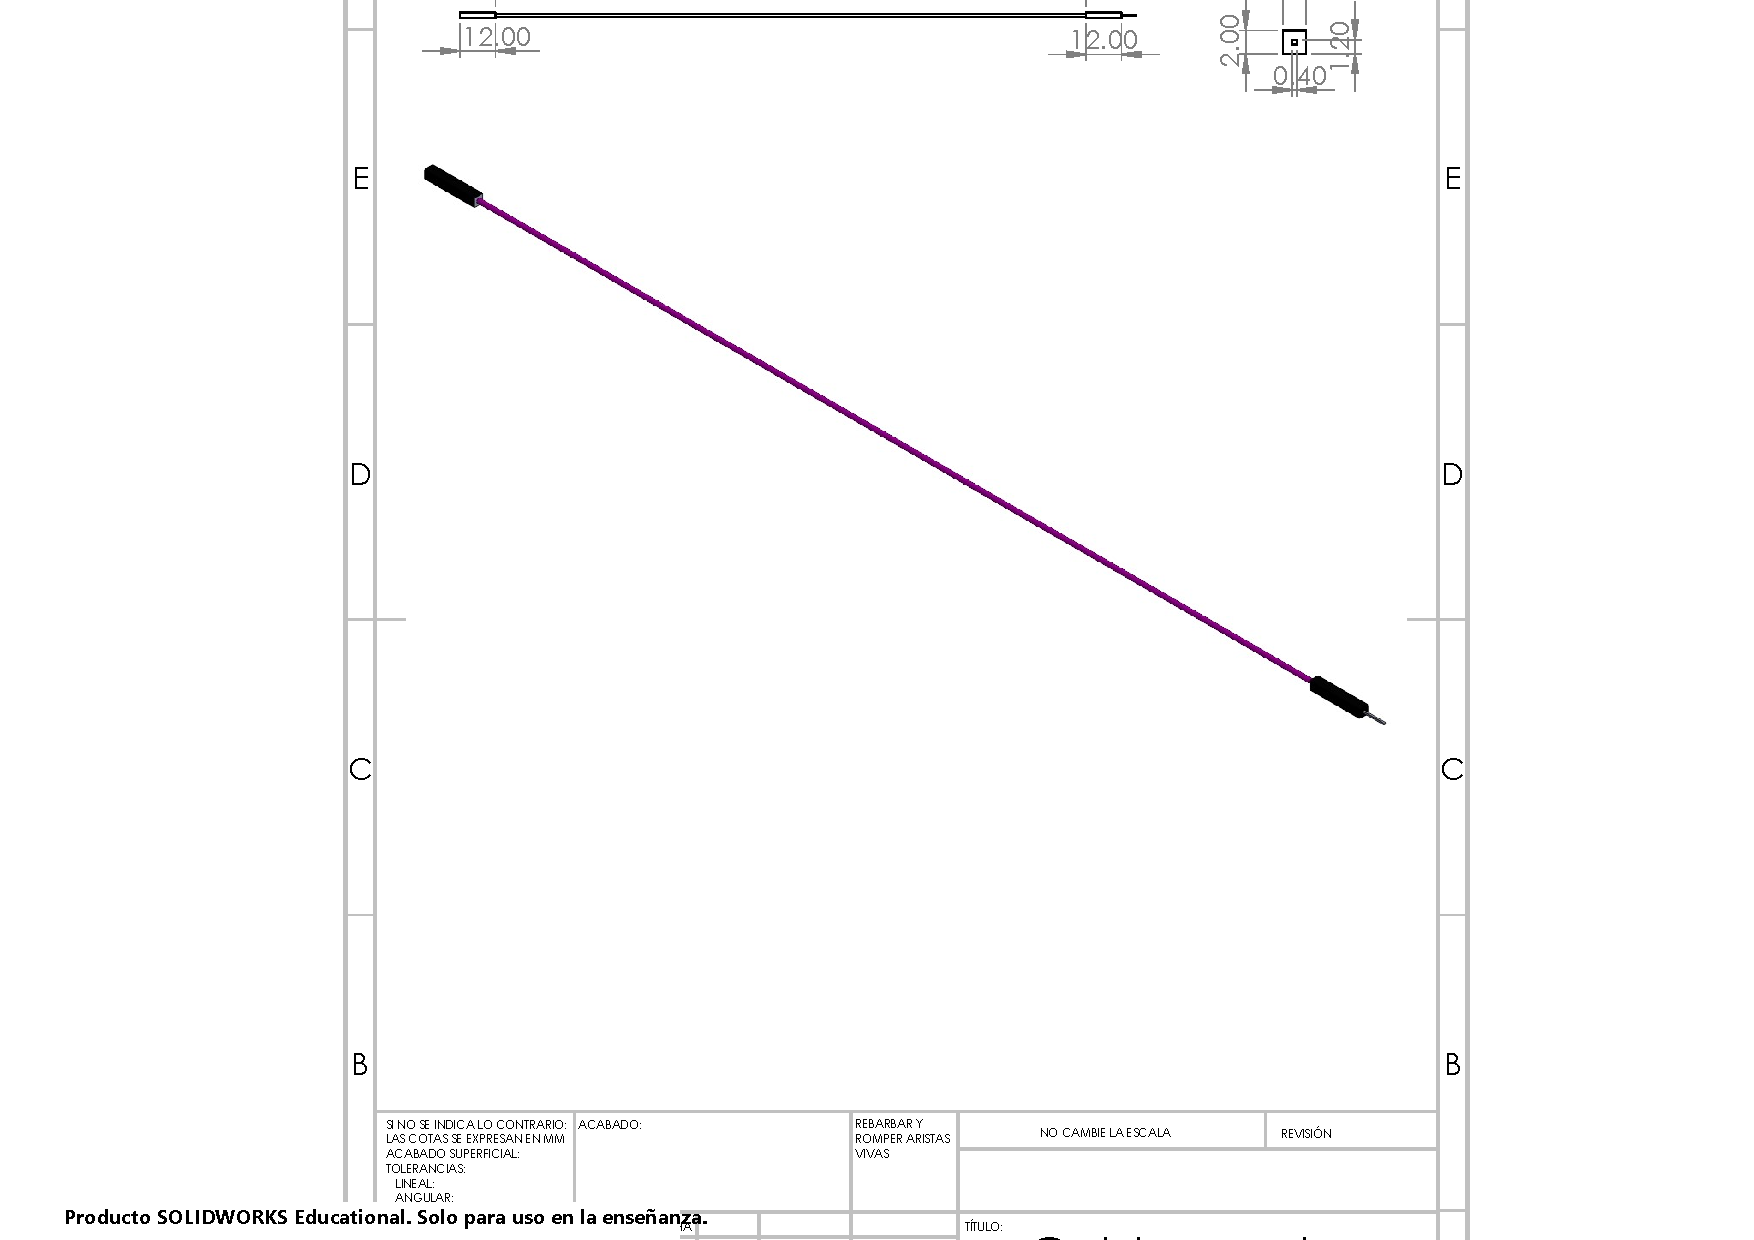
\includegraphics[trim = {10mm 10mm 10mm 10mm},clip,scale=0.5]{23/img/Cable macho-hembra 5v..pdf}
        \caption{Croquis cable macho}
        \label{fig:lcd-16x2}
    \end{figure}
    %
    %
    % 
    % 
    \begin{figure}[H]
        \centering
        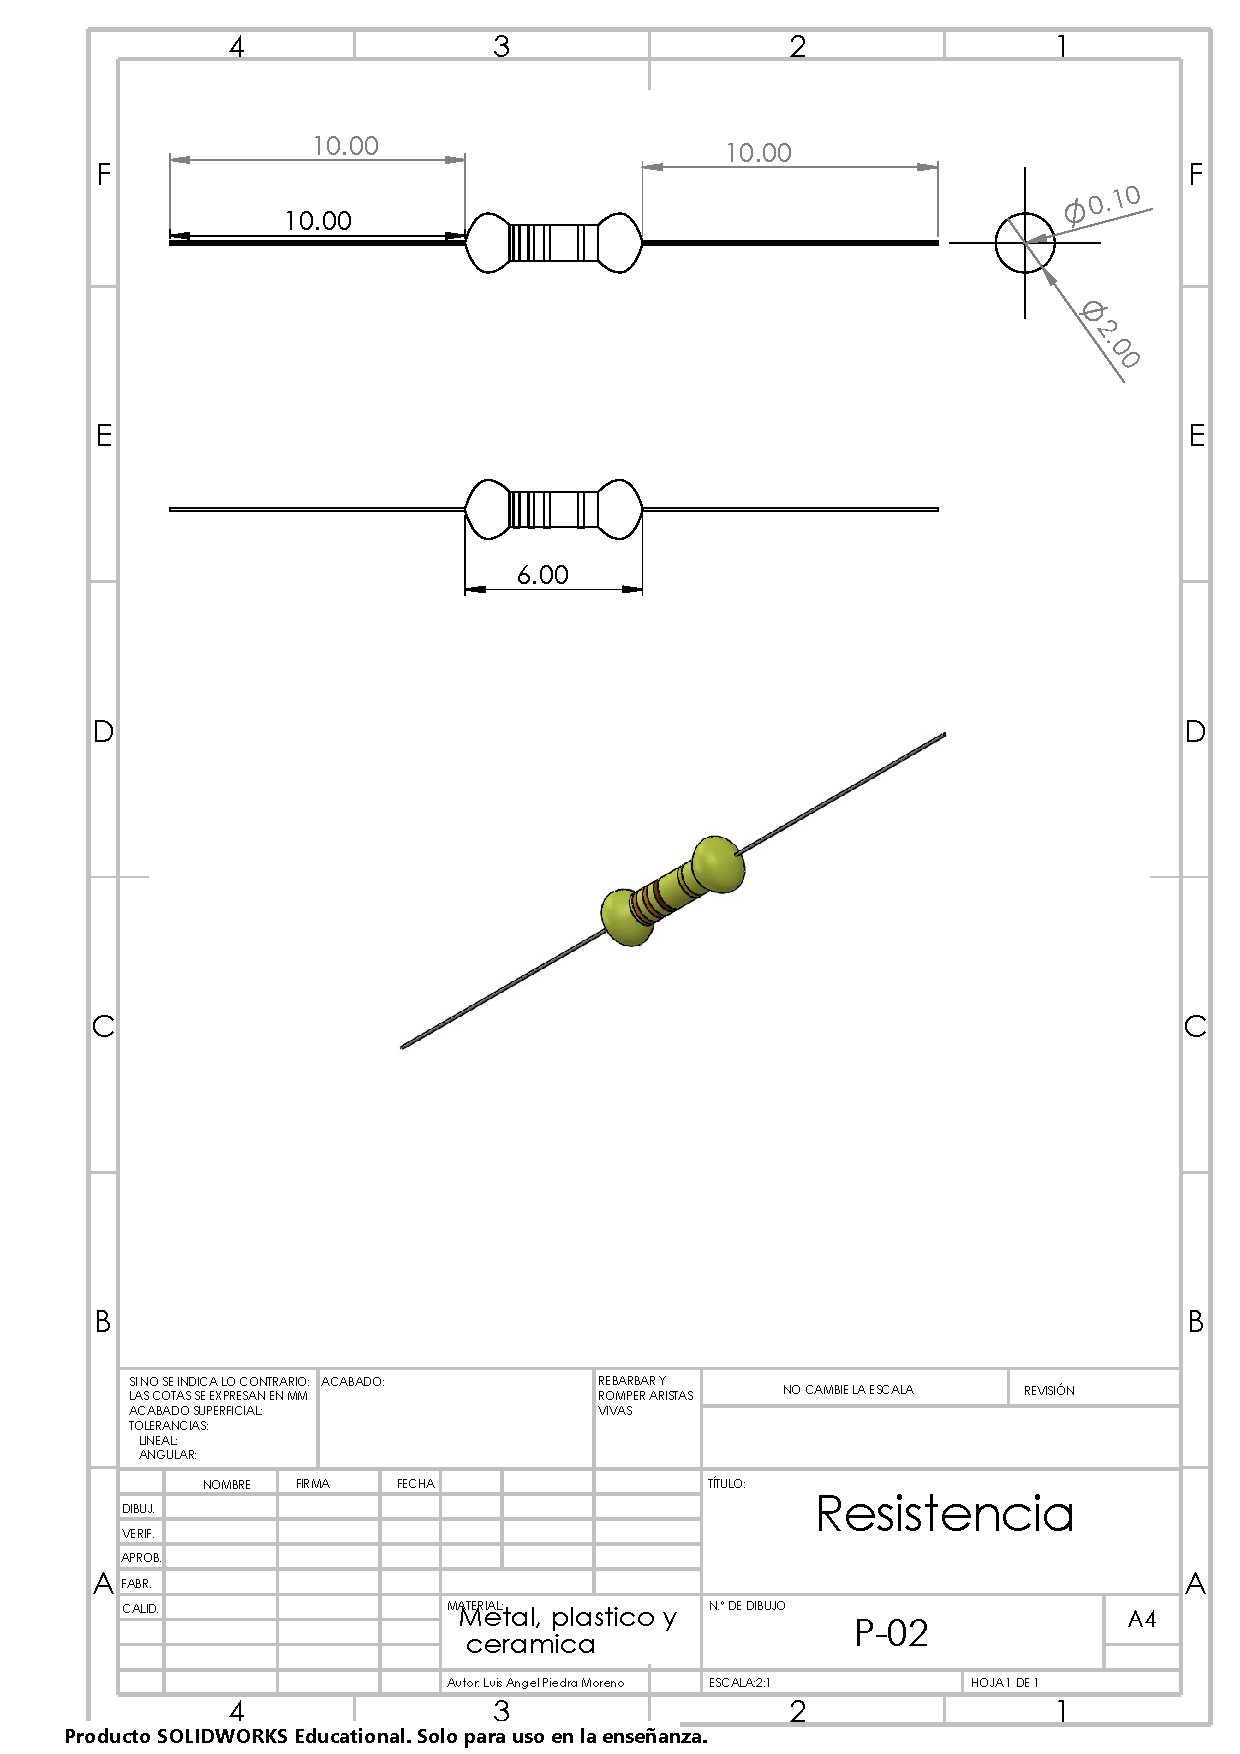
\includegraphics[trim = {10mm 10mm 10mm 10mm},clip,scale=0.2]{23/img/Resistencia.pdf}
        \caption{Croquis Resistencia}
        \label{fig:lcd-16x2}
    \end{figure}
    % 
    % 
    % 
    % 
    \begin{figure}[H]
        \centering
        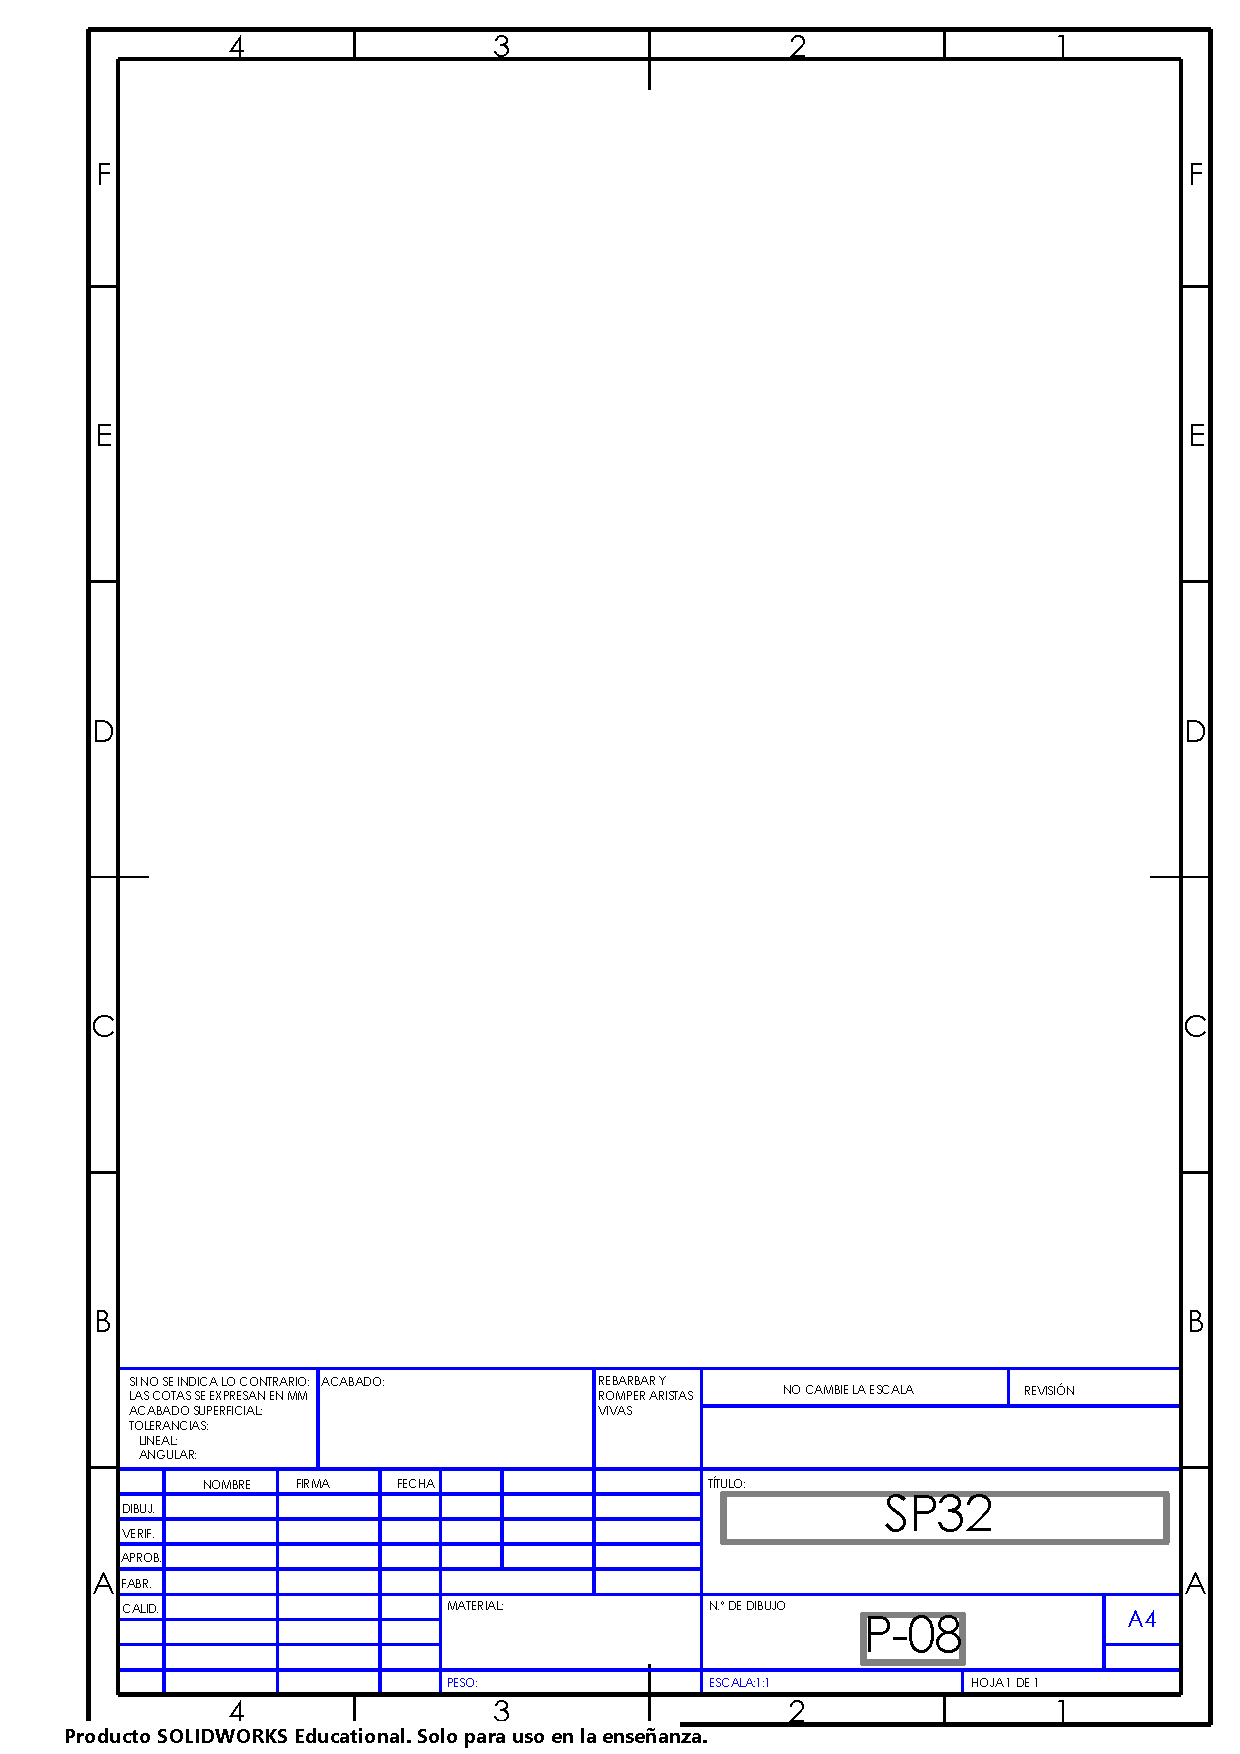
\includegraphics[trim = {10mm 10mm 10mm 10mm},clip,scale=0.2]{23/img/SP32.pdf}
        \caption{Esquema SP32}
        \label{fig:lcd-16x2}
    \end{figure}
    % 
    % 
    % 
    % 
    \begin{figure}[H]
        \centering
        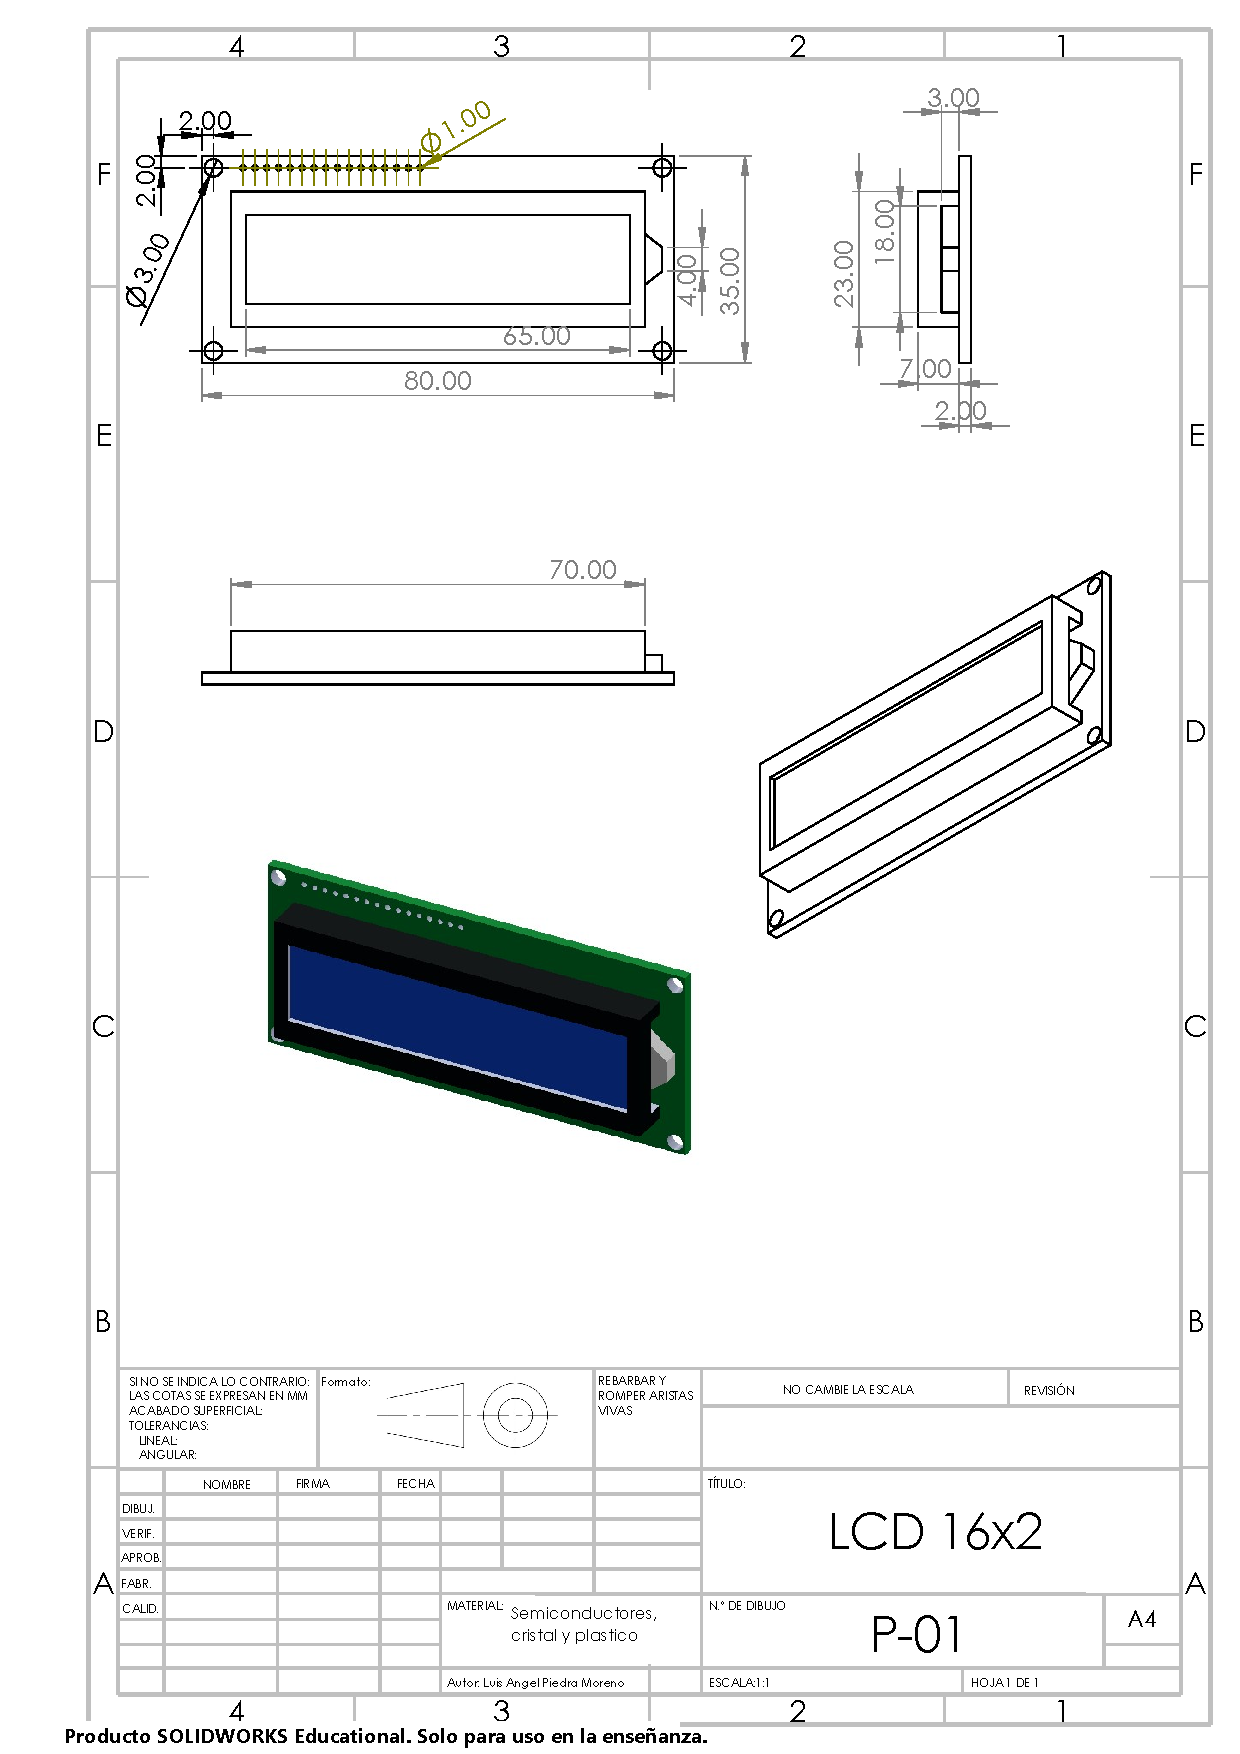
\includegraphics[trim = {10mm 10mm 10mm 10mm},clip,scale=0.2]{23/img/LCD2.pdf}
        \caption{Croquis LCD}
        \label{fig:lcd-16x2}
    \end{figure}
    % 
    % 
    % 
    % 
    \begin{figure}[H]
        \centering
        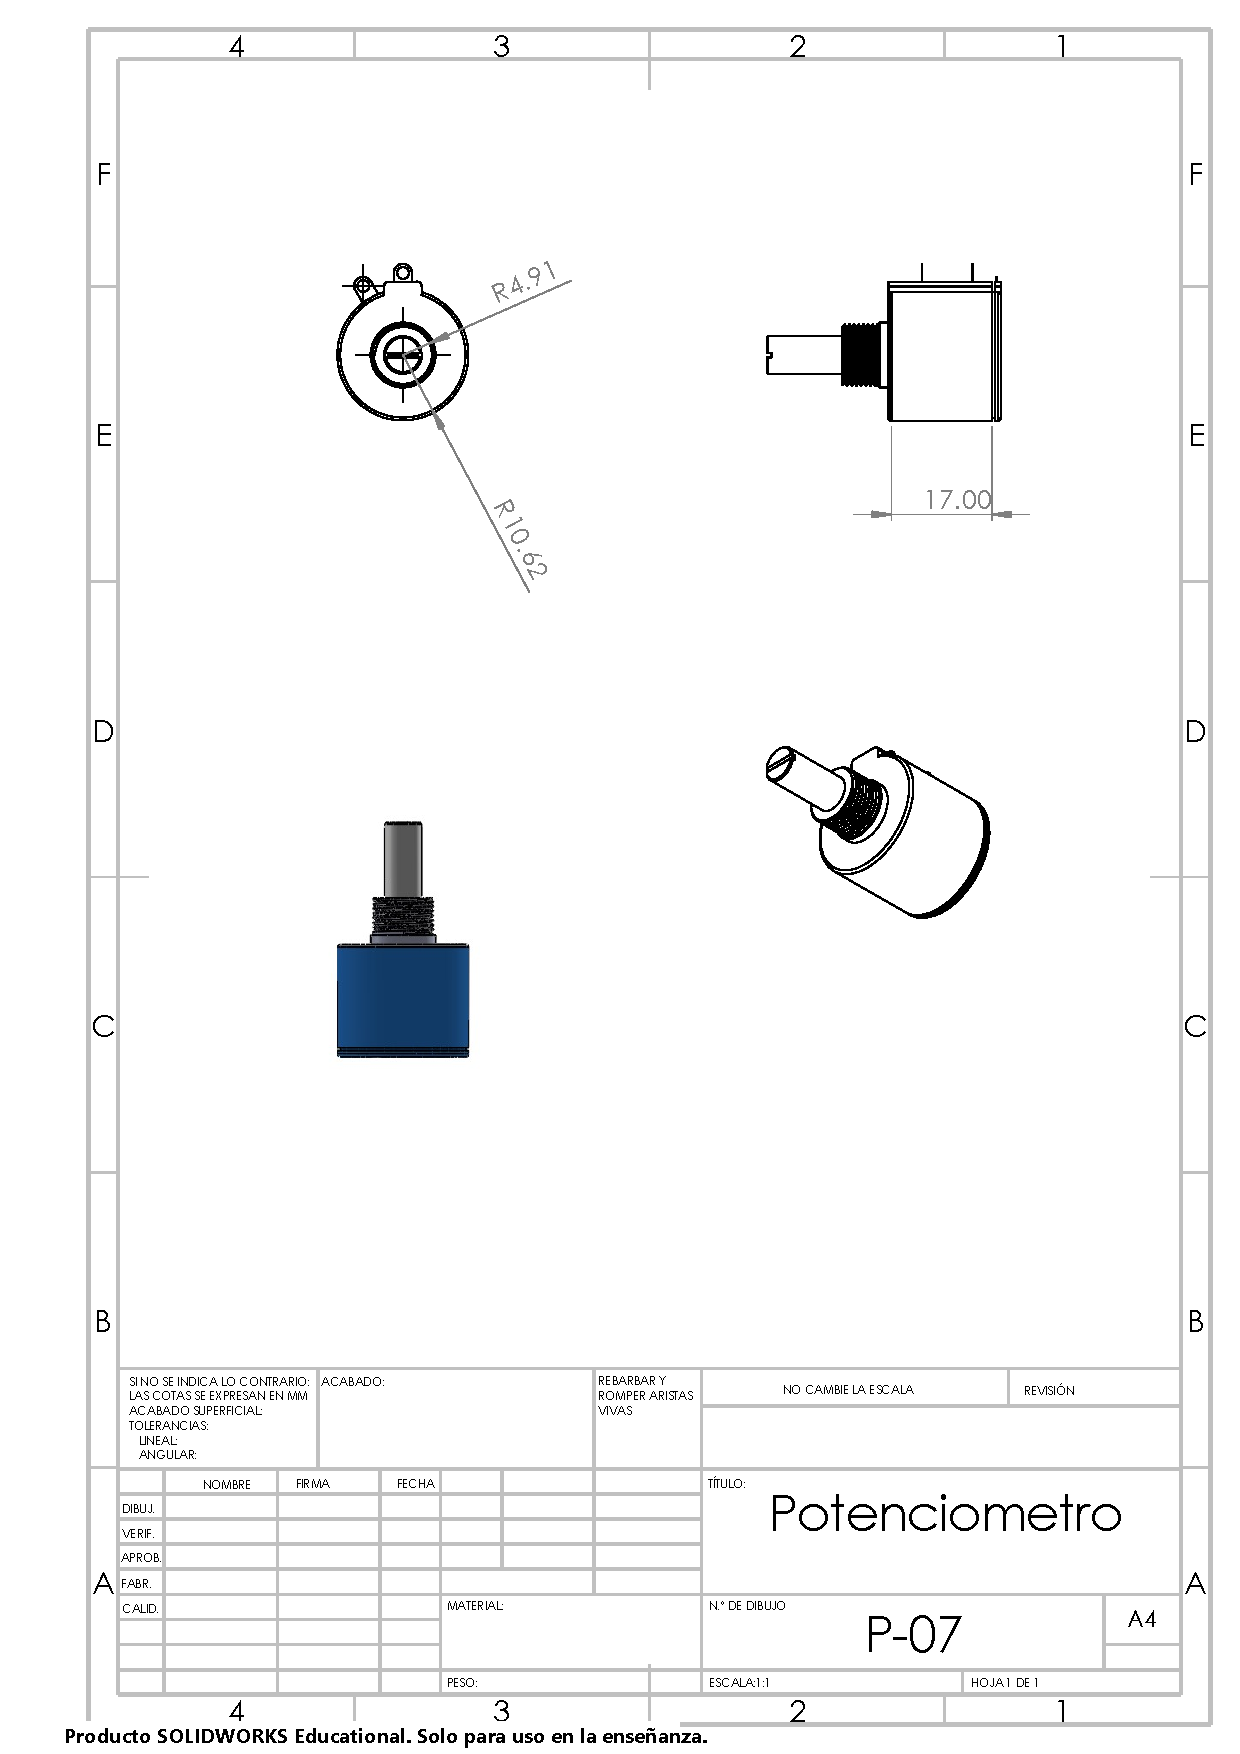
\includegraphics[trim = {10mm 10mm 10mm 10mm},clip,scale=0.05]{23/img/Potenciometro.pdf}
        \caption{Croquis Potenciometro}
        \label{fig:lcd-16x2}
    \end{figure}
    % 
    % 
    % 
    % 
    \begin{figure}[H]
        \centering
        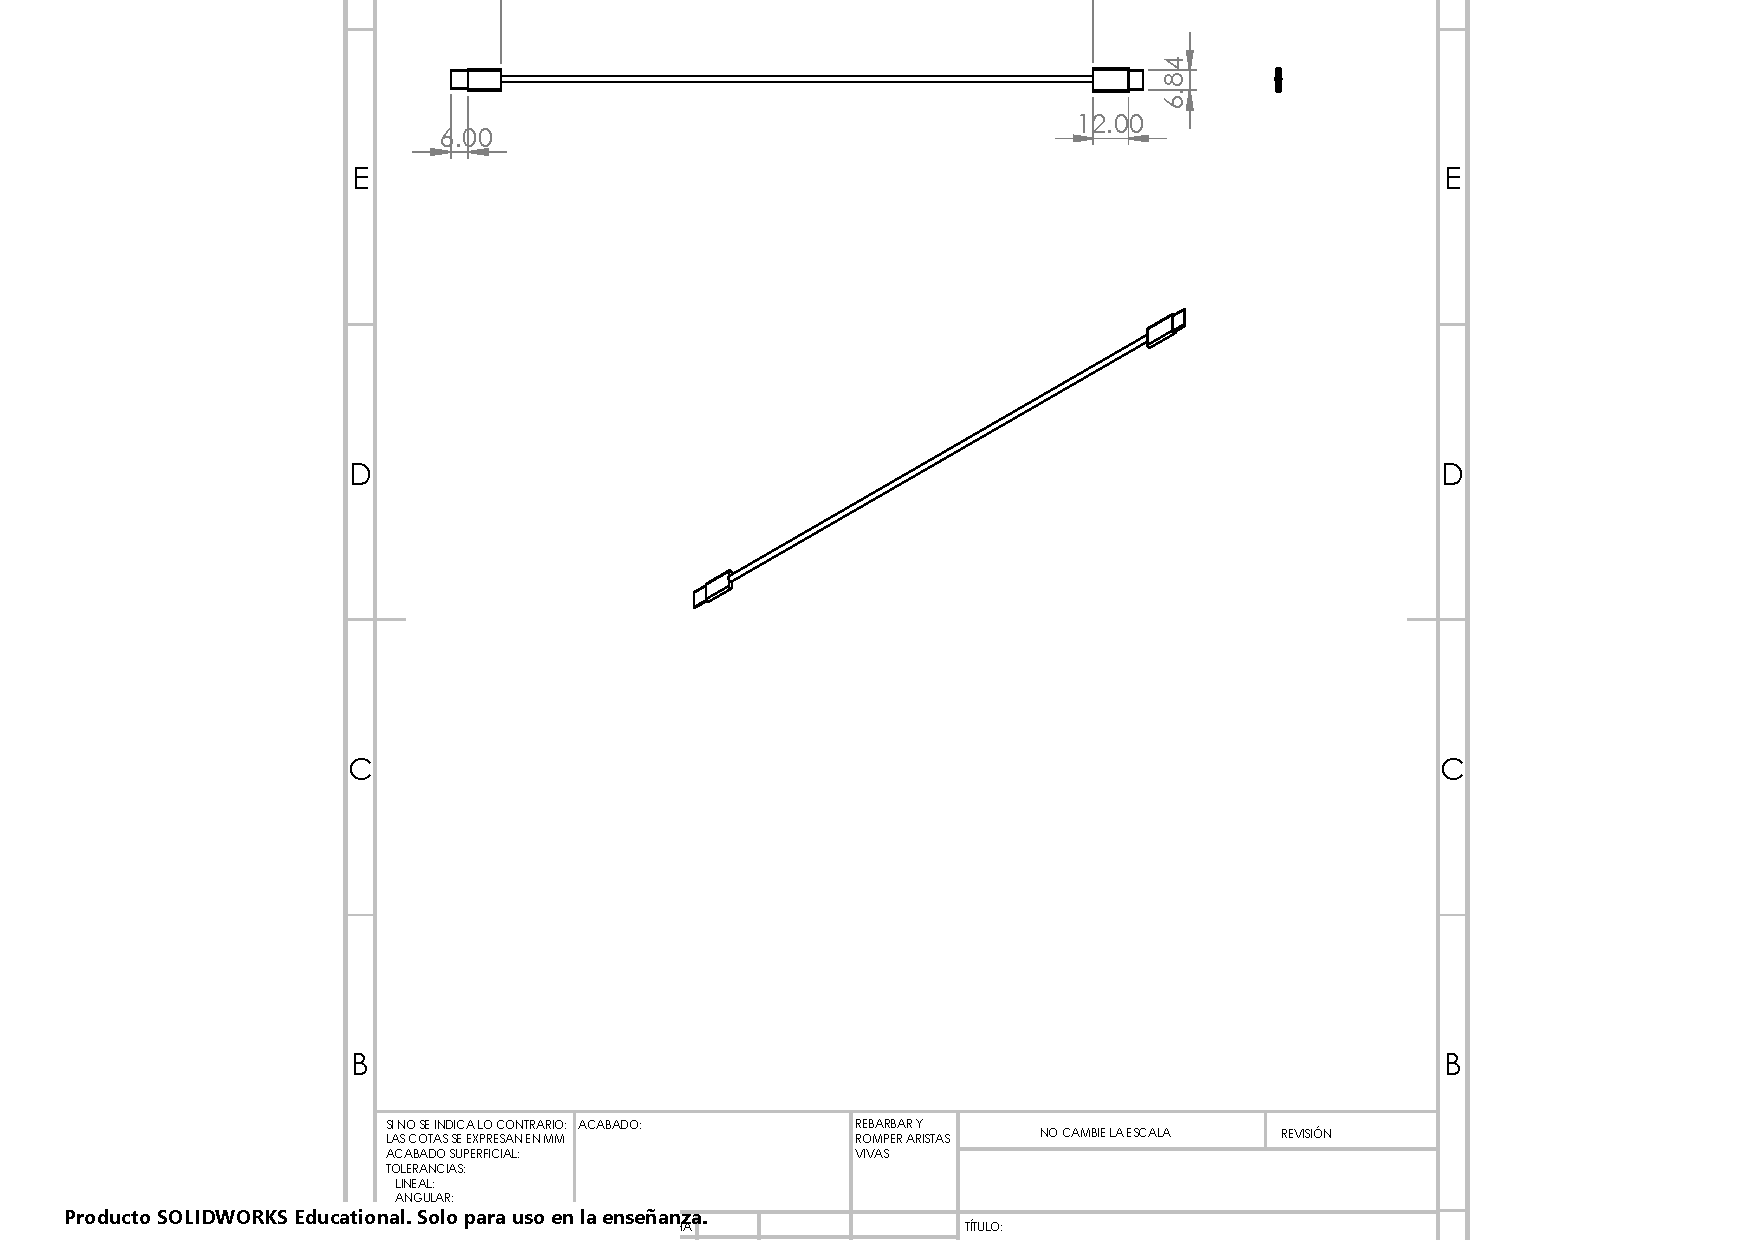
\includegraphics[trim = {10mm 10mm 10mm 10mm},clip,scale=0.2]{23/img/cable usb c.pdf}
        \caption{Esquema Potenciometro}
        \label{fig:lcd-16x2}
    \end{figure}
    % 
    % 
    \subsection{Prepara tu documento}
    
    Antes de que comiences a utilizar esta plantilla, es recomendable que prepare la información que contendrá en un archivo aparte. 
    Ten preparadas tus gráficas, así como también las tablas aparte, para que sea más fácil integrarlo. 
    Se recomienda fuertemente el uso de \textbf{formato Enhanced Metafile (.emf) para imágenes y gráficas} de resolución óptima. 
    Finalmente, completa y organiza el contenido antes de darle el formato de esta plantilla. 
    
    \subsection{Acrónimos y Abreviaciones}
    
    Los acrónimos y abreviaciones deberán ser definidos únicamente la primera vez que aparecen en el texto, esto para que el lector entienda lo que significan.
    
    \subsection{Ecuaciones}
    
    Las ecuaciones son una excepción a las especificaciones prescritas de esta plantilla. 
    Deberá determinar si su ecuación debe escribirse o no utilizando la fuente Adobe Devangari. 
    Para crear ecuaciones multinivel, puede ser necesario tratar la ecuación como un gráfico e insertarla en el texto después de aplicar el estilo de la platilla.
    Las ecuaciones serán enumeradas de manera consecutiva, y el número de ecuación, entre paréntesis, se colocan al ras de la derecha, utilizando una tabulación derecha. 
    
    \begin{equation}
        \label{eq1}
        x + y = z 
    \end{equation}
    
    Es importante asegurarse de que los símbolos de la ecuación sean definidos antes o inmediatamente después de la ecuación. Utilice “(1)”, en vez de “Eq. 1” al enumerar las ecuaciones, excepto al principio de una oración: “La ecuación (\ref{eq1}) es…”
    
    \section{Resultados y discusión}
    
    Antes de comenzar a preparar tu artículo, es importante que lea primero la guía del autor, la cual incluye los temas o apartados que son necesarios para tener tu trabajo completo.
    Una vez completada la edición del texto, el documento está listo para el uso de esta plantilla. En este archivo recién creado, resalte todo el contenido e importe el archivo de texto preparado. Ahora esta listo para estilizar su documento.
    En esta sección se deben presentar todo lo obtenido de la sección 2, incluidas deducciones o efectos del desarrollo. También se podrán incluir subsecciones numeradas de la siguiente forma:
    
    \subsection{Autores y Afiliaciones}
    
    Para distinguir las afiliaciones de los autores, utilice superíndices iniciando con el número 1, 2, etc., sucesivamente, esto dependerá de la cantidad de los departamentos a los que estén afiliados los autores. En caso de que todos los autores pertenezcan a una mismo departamento e institución, utilizar sólo el superíndice 1. 
    
    \subsection{Identificar los encabezados}
    
    Se les recuerda a los autores que los encabezados deben de estar conforme los solicita la guía del autor. De ahí se puede adaptar el trabajo para que sea más fácil de entender para el lector.
    Los encabezados organizan los temas sobre una base relacional y jerárquica. Por ejemplo, el título del documento es encabezado del texto principal porque todo el material posterior se relaciona y elabora sobre este tema. 
    
    \subsection{Tablas y Figuras}
    
    \begin{enumerate}
        \item Posición de las tablas y figuras: Coloque las figuras y las tablas en la parte superior e inferior de las columnas. Evite colocarlos en medio. Las figuras y las tablas grandes pueden abarcar ambas columnas. Los títulos de las figuras deben de estar debajo de las mismas; los títulos de las tablas deben aparecer encima de ellas. Insértese las figuras y los cuadros después de citarse en el texto. Utilice la abreviatura “Fig. 1”, incluso al principio de una oración. 
    \end{enumerate}
    
    \section{Conclusiones}
    
    Se describe aquí el alcance del trabajo, logros obtenidos y perspectivas para el futuro de este. Se sugiere colocar información cuantitativa obtenida.
    
    \section{Agradecimientos}
    
    Es importante darles su debido reconocimiento a los laboratorios, instituciones, organizaciones, entre otros que han sido participes para la culminación de este trabajo. También es importante mencionar, fondos, proyectos, becas, entre otros que se le han otorgado al o los autores para realizar el trabajo de investigación. Ejemplo: “Los autores agradecen al Concejo Nacional de Ciencia y Tecnología por los recursos otorgados…”
    
    \section*{Referencias}
    
    Para esta platilla, se solicita al autor enumerar las citas de manera consecutiva entre corchetes \cite{YLi2013}. 
    La puntuación de la oración que sigues sería \cite{Mesaelides2011}. 
    Refiérase simplemente al número de referencia, como en \cite{Morales2012}, no utilice “Ref. [3]” o “referencia [3]” excepto al principio de una oración: “La referencia [3] fue la primera…”
    Enumere las notas al pie por separado en superíndices. Coloque la nota de pie de en la parte inferior de la columna en la que se citó. No coloque notas al pie en la lista de referencias. Utilice letras para las notas al pie de la tabla.
    A menos de que haya tres autores o más; no utilice “et al.”. Los trabajos que no hayan sido publicados, incluso si han sido presentados para su publicación, deben ser citados como “inéditos”. Los trabajos que han sido aceptados para su publicación deben de citarse como “en prensa”. Poner en mayúscula sólo la primera palabra de un título, excepto los nombres propios y los símbolos de elemento. 
    Otros ejemplos \cite{LAAngeles2021}, \cite{LAAngelesConni}. 
    Véase el link \cite{prueba}.
    
    % Ejemplo
    %  @Article{article,
    % 	author = "Author1 LastName1 and Author2 LastName2 and Author3 LastName3",
    % 	title = "Article Title",
    % 	volume = "30",
    % 	number = "30",
    % 	pages = "10127-10134",
    % 	year = "2013",
    % 	doi = "10.3389/fnins.2013.12345",
    % 	URL = "http://www.frontiersin.org/Journal/10.3389/fnins.2013.12345/abstract",
    % 	journal = "Frontiers in Neuroscience"
    % }
    
    % @book{book,
    %   author    = {Author Name}, 
    %   title     = {The title of the work},
    %   publisher = {The name of the publisher},
    %   address   = {The city},
    %   year      = 1993,
    % }
    
    % @incollection{chapter,
    %   author       = {Bauthor Surname}, 
    %   title        = {The title of the work},
    %   editor       = {Editor Name},
    %   booktitle    = {The title of the book},
    %   publisher    = {The name of the publisher},
    %   address      = {The city},
    %   year         = 2002,
    %   pages        = {201-213},
    % }
    
    % @InProceedings{conference,
    %   author = {Cauthor Name and Dauthor Surname and Fauthor LastName},
    %   title = {The title of the work},
    %   booktitle = {The title of the conference proceedings},
    %   year = 1996,
    %   publisher = {The name of the publisher},
    %   editor = {Editor Name1 and Editor Name2},
    %   pages = {41-50},
    % }
    
    % @book{cho,
    %   author       = {Gauthor Name1}, 
    %   title        = {The title of the work},
    %   publisher = {Country code and patent number},
    %   address      = {Patent Country},
    %   year = 2013
    % }
    
    % @book{patent,
    %   author    = {Hauthor Surname1}, 
    %   title     = {The title of the work},
    %   publisher = {Patent number},
    %   address   = {Patent country},
    %   year      = 2010,
    % }
    
    % % please use misc for datasets
    % @misc{dataset, 
    % 	author = "Author1 LastName1 and Author2 LastName2 and Author3 LastName3",
    % 	title = "Data Title",
    % 	year = "2011",
    % 	doi = "10.000/55555",
    % 	URL = "http://www.frontiersin.org/",
    % }
    
    \bibliographystyle{ieeetr}
    \bibliography{23/referencias}
    % 
    % 
    %%%%%%%%%%%%%%%%%%%%%%%%%%%%%%%%%%
    \appendix
    %%%%%%%%%%%%%%%%%%%%%%%%%%%%%%%%%%
    % 
    % 
    \centering{\section[\appendixautorefname{}]{Apéndice}}\label{anexo:pines}
    \includepdf[pages=-]{23/img/Conectar la extensión al enchufe.pdf}
    %%%%%%%%%%%%%%%%%%%%%%%%%%%%%%%%%%%%%%%%
    \newpage
     \bibliographystyle{ieeetr}
        \bibliography{23/referencias}